\section{Purpose}
The primary science purpose of the dissertation research is to use meticulous and systematic observational evidence to clarify the physical connections between Alfvénic auroral morphologies and ionospheric turbulence that produces coherent ISR backscatter.
The dissertation work resulted in a multi-station synchronized observatory recording auroral video at \unit[20]{ms} cadence.
As described in section~\ref{sec:fuspfisr} and chapter~\ref{chapter:sim}, this cadence is adequate for detecting and characterizing the associations between Langmuir turbulence and Alfvénic aurora.

Plasma traveling throughout the solar system and bound to planetary bodies is constantly subjected to changing magnetic field configurations and bulk flows.
A streaming instability results when a locally strong flow of particles (current), such as electronic precipitation into the ionosphere, causes longitudinal waves in the background plasma. 
Under frequently occurring conditions, the plasma wave grows exponentially into a streaming instability.
The ionospheric turbulence creates signatures readily detected by sufficiently fast sampling ISR and synchronized camera systems, allowing distinction between various types of Alfvén wave-sourced perturbations and characterization based on remote sensing inversion algorithms as developed in chapters~\ref{chapter:sim} and \ref{chapter:fusion}.

Each important aspect of the sensing system design and implementation is described to allow reproduction of the experimental apparatus and build confidence in the character of its output products.
Section~\ref{sec:aurorabasic} introduces key facets of optical auroral observation and processing advanced by the dissertation, expanded upon in chapter~\ref{chapter:inst}.
Section~\ref{sec:isrbasic} introduces connections between ISR and HiST optical observations and inversion, expanded upon in chapter~\ref{chapter:fusion}.
The necessary algorithms created to detect Alfvénic aurora and ion-acoustic turbulence seen in radar are introduced in section~\ref{sec:intdiscrim} and described in chapter~\ref{chapter:discrim} with additional applications showing the generality of the technique in appendices~\ref{chapter:marsis} and \ref{chapter:passive}.

\FloatBarrier
\subsection{Characterizing sources of fine-scale auroral structure}\label{sec:aurorabasic}
The optically thin aurora with observed optical intensity $\mathscr{I}$ due to auroral volume emission rate (VER) $p$ looking along direction $\vect{r}$ is described by
\begin{equation}\label{eq:bint}
\mathscr{I} = \int_0^\infty p(\vect{r})\textrm{d}\vect{r}
\end{equation}
implying that ground-observed auroral brightness strongly depends upon viewing angle.
Additional important factors such as wavelength-dependent atmospheric absorption between the aurora and observer are detailed in chapter~\ref{chapter:sim}.
Non-uniqueness of the observational system is implicit in (\ref{eq:bint}) as demonstrated with the examples in Figure~\ref{fig:bint} for an optically thin 2-D phantom. 
\begin{figure}\centering
    \begin{subfigure}[t]{0.45\linewidth}\centering
        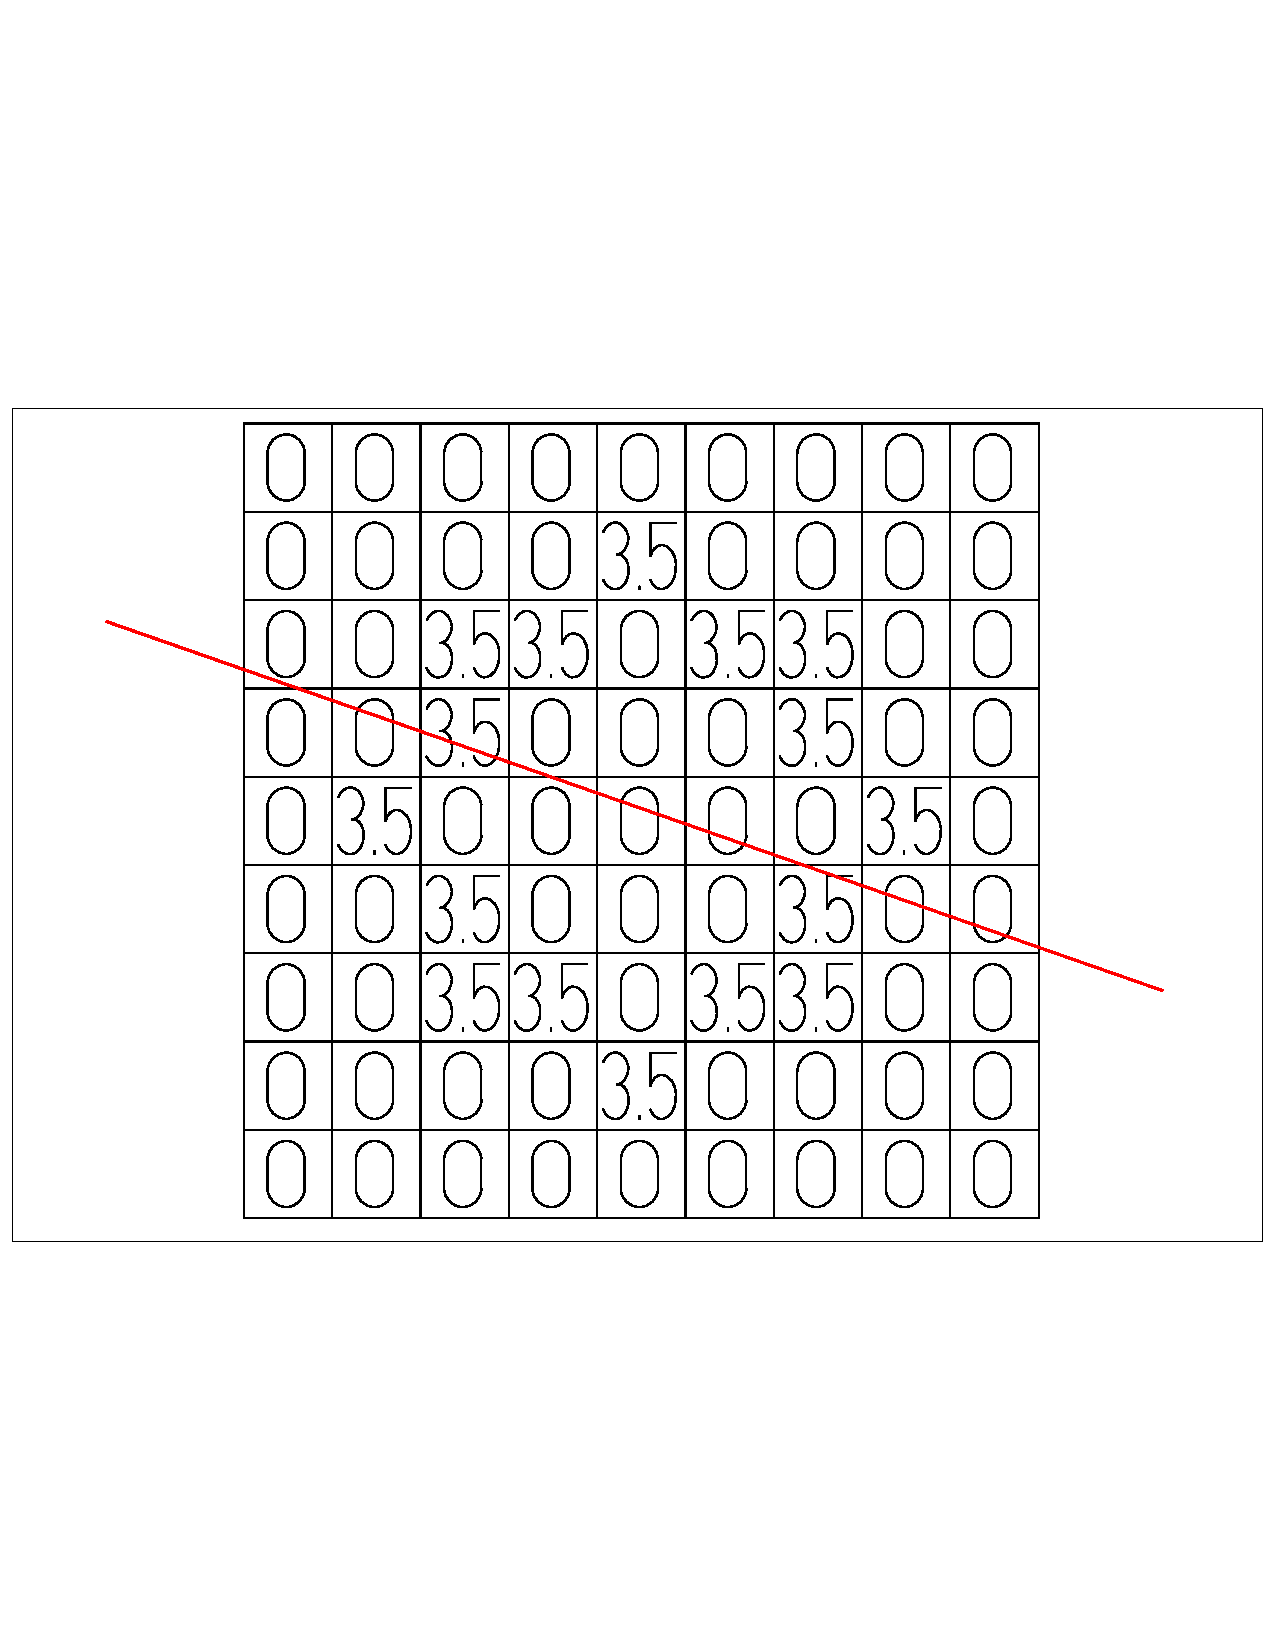
\includegraphics[width=\linewidth,trim=50 200 50 200,clip]{gfx/circle}
        \caption{Hollow optically thin structure with line-of-sight.}		
    \end{subfigure}
    \begin{subfigure}[t]{0.45\linewidth}\centering
        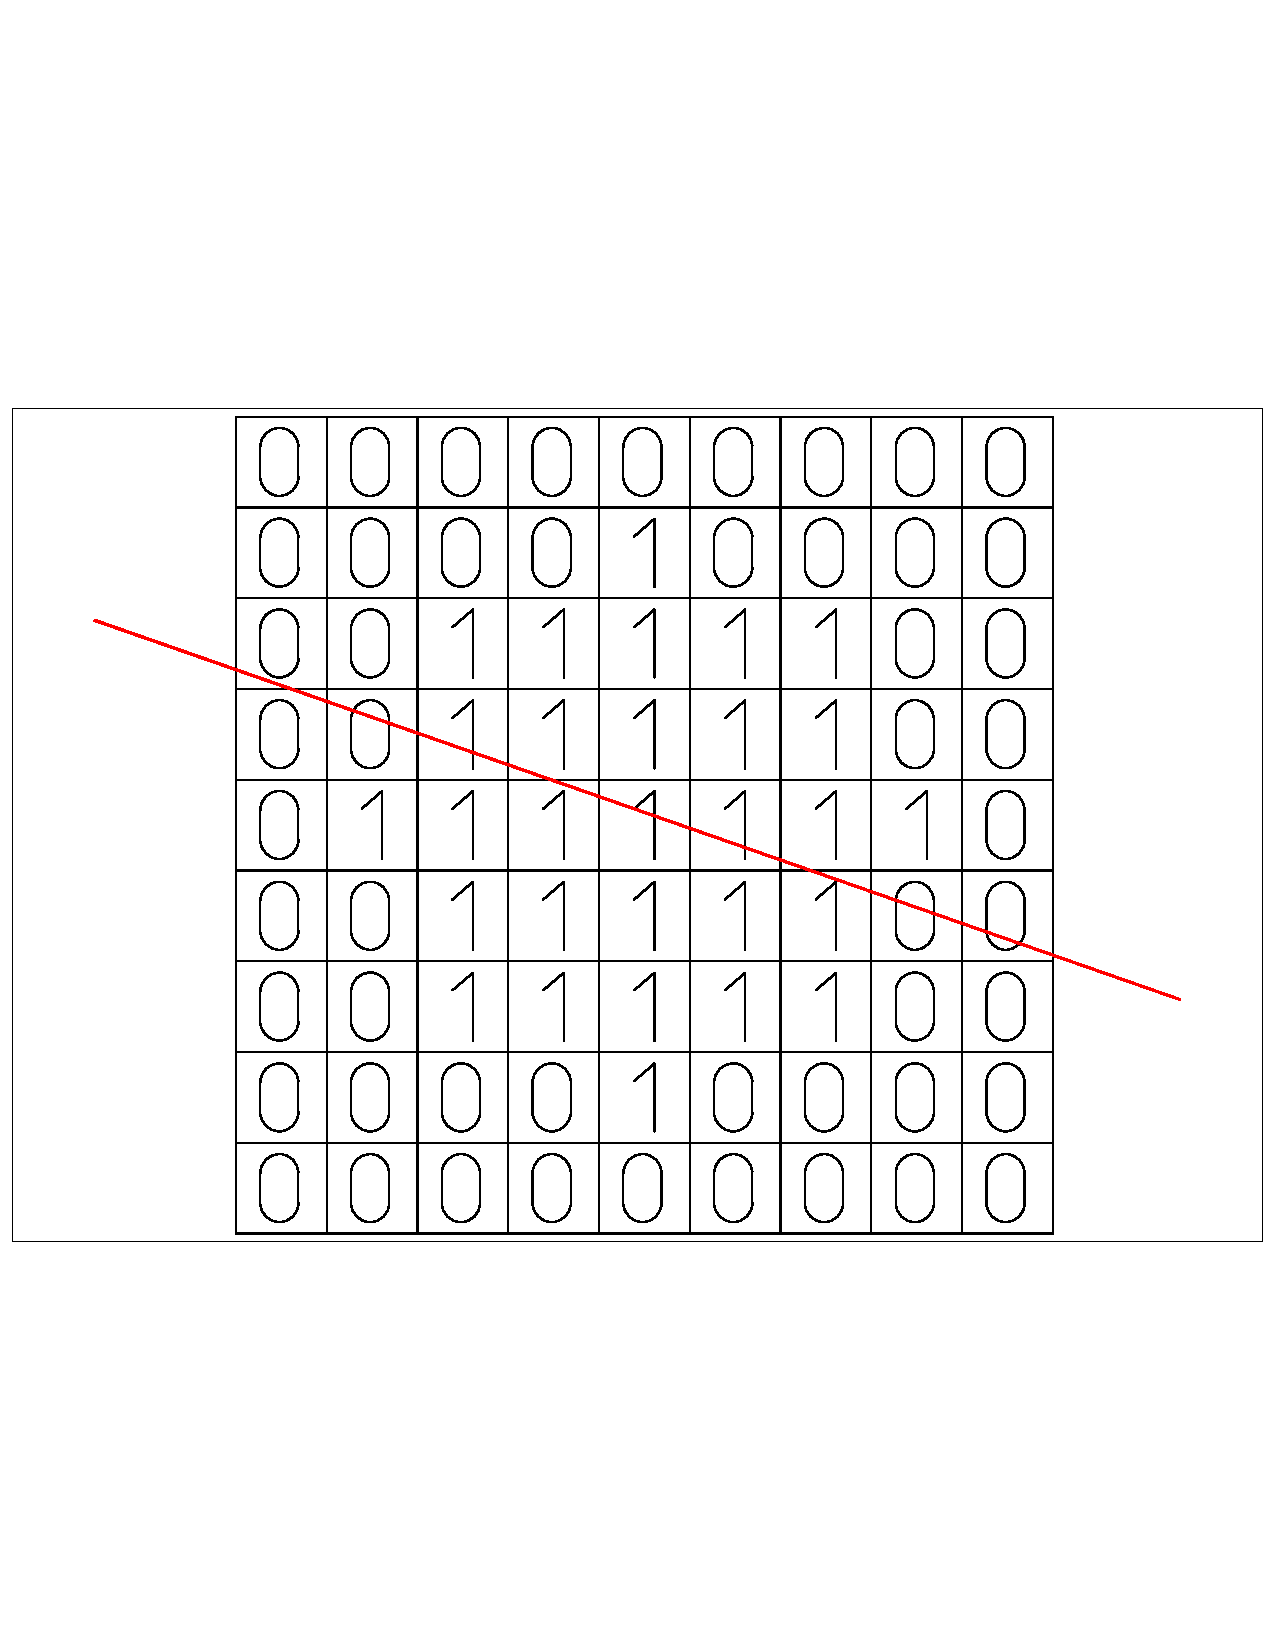
\includegraphics[width=\linewidth,trim=50 200 50 200,clip]{gfx/disk}
        \caption{Filled optically thin structure with line-of-sight.}		
    \end{subfigure}
    \caption{Optically thin phantoms with red line-of-sight integral. Completely distinct forms after line-integration give the same result, an example of the non-uniqueness problems inherent to auroral remote sensing.}\label{fig:bint}
\end{figure}
Whether the observed target is disk, circle, spline or other arbitrary form, line integration of distinct forms can lead to the same integrated (observed) result.

We assume the auroral cameras are boresight-aimed at magnetic zenith. 
Non-uniqueness becomes increasingly important for large camera viewing angle from magnetic zenith $\theta \gg \unit[1]{degree}$.
As camera ground spacing increases beyond $x \sim \unit[10]{km}$ increasingly poor resolution of fine detail along $B_\perp$ results as demonstrated in Figure~\ref{fig:camres}.
\begin{figure}
	\begin{subfigure}[t]{0.45\linewidth}\centering
		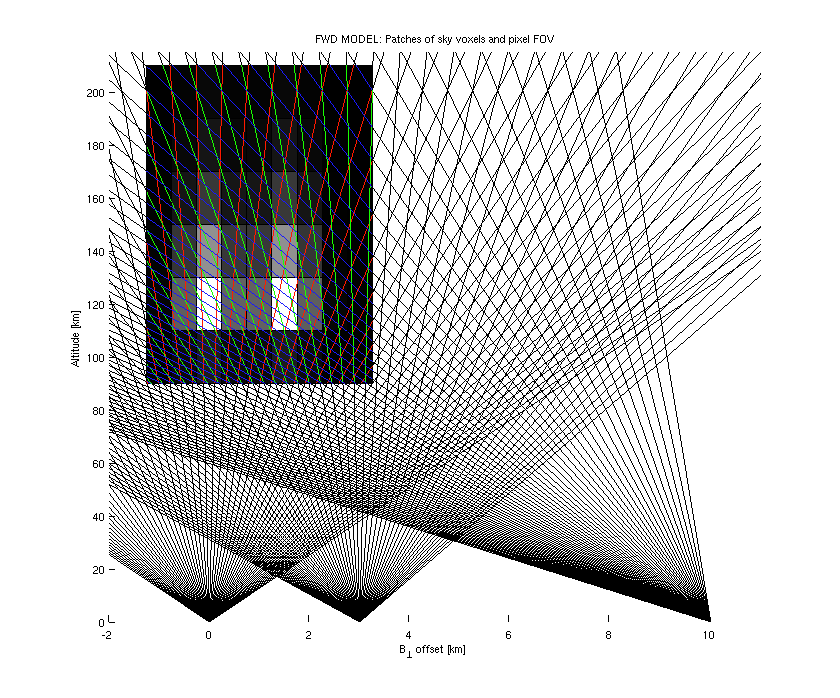
\includegraphics[width=\columnwidth]{../gfx/L3cam}
		\caption{Viewing geometry for auroral arc with cameras at $x \in (0,3,10)$~km.}
	\end{subfigure}
	\begin{subfigure}[t]{0.45\linewidth}\centering
		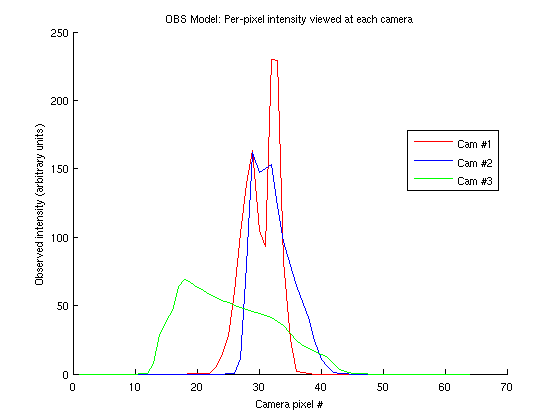
\includegraphics[width=\columnwidth]{../gfx/I3cam}
		\caption{Intensity $I$ for three cameras.}
	\end{subfigure}
	\caption{Notice how the intensity of the green line for $x=\unit[10]{km}$ has smeared out the \unit[1.5]{km} spaced arcs, demonstrating a non-uniqueness issue.}
	\label{fig:camres}
\end{figure}
Figure~\ref{fig:camres}(b) shows the non-uniqueness issue in auroral tomography, particularly for cameras widely spaced from the auroral arc of interest.
Alfvénic splitting auroral arcs with widths in the \unit[0.01..1]{km} range are best observed with cameras spacing $x < \unit[10]{km}$.

The diverse colors and shapes of the aurora have been the focus of human study and speculation for centuries.
The colors of the aurora consist of isolated spectral lines, close groups of spectral lines and continua of spectral bands.
Auroral optical emissions are photons released as excited particles (atoms and molecules, ions and neutrals) relax and emit a photon with wavelengths determined by quantum physics.
The precipitating electron energy at the top of the ionosphere likewise varies between monoenergetic, a band-limited uniform spectrum or a complex spectrum having one or more peaks in a broadband differential number flux spectrum.
% NOTE: example figure here?
Precipitating particle sources include electrons mirroring in the upper ionosphere, particles ejected from the plasma sheet or launched from the magnetotail.
More important to this work than where the electron came from is what acceleration process the particle experienced before crashing into the ionosphere.
Alfvén wave accelerated particles have key signatures in the differential number flux spectrum.
Alfvén wave accelerated electrons kinetically reacting with E- and F-region ionospheric particles give particular signatures in high-speed auroral and ISR observations that are connected observationally in this dissertation.
These factors imply that an appropriate inversion algorithm may yield new science conclusions about the association and characteristics of Alfvénic aurora and plasma turbulence.

Essential to the analyses in this dissertation is the fact that auroral behavior in the $B_\parallel$ dimension may be modeled by numerical solutions to partial differential equations describing energy deposition along a flux tube.
The important \textit{a priori} inputs to such models include solar zenith angle (SZA) (that is, angle of the sun from local zenith).
SZA is commonly used in auroral studies because of the inherent angular ambiguity near the horizon due to refraction. 
When the sun is seen to be at the horizon, the sun is already geometrically below the horizon under typical conditions.
During the day, photodissociation due to solar EUV gives rise to the D-layer ionosphere, absorbing MF.
During solar energetic particle events lower HF wavelengths are also absorbed.

Neutral atoms and molecules along with ions are a prerequisite for structured aurora.
These ionospheric particles are impacted by electrons in finely structured (in $B_\perp$) beams to create structured aurora.
Just before Sputnik I was launched, \citet{chamberlain1957} raised the possibility that locally-accelerated electrons were responsible for fine auroral structure in the E-region, while prior work such as \citet{seaton1954} suggested electrons could not generate E-region aurora.
The first group of Sputnik and Explorer spacecraft in 1957--1958 made structured proton aurora in the E-region seem unlikely and a local acceleration mechanisms for electrons probable \citep{krassovsky1959,wallace1959}.
The primary role of the electron in structured E-region aurora was solidly established by 1960 with \textit{in situ} sounding rocket sensors of increasing fidelity revealing typical scales and dynamics of auroral precipitation.
Of note are the pair of \unit[120]{km} apogee sounding rockets \citep{mcilwain1960} determining the important result that proton particle flux was $\ll 1\%$ electron particle flux, electron energy flux was at least 10 times that of proton energy flux, and small amounts of differential number flux were found.
1963 satellite measurements \citep{sharp1965} at $\unit[8]{ms} \Leftrightarrow \unit[63]{m}$ sampling cadence showed rapidly changing energy spectrum amidst a more slowly changing energy flux.
These observations confirmed that most of the auroral flux had particles less than \unit[10]{keV} with the largest differential number flux at energies $\ll \unit[1]{keV}$.

\subsubsection{Objectives related to characterizing sources of fine-scale auroral structure}
\citet{chaston2007how} noted the characteristics of Alfvénic aurora consistent with the design of the HiST system \citep{hirsch2016}.
The following HiST performance metrics were vital to success:
\begin{enumerate}
	\item Observe aurora with cadence $\leq\unit[20]{ms}$
	\item Operate unattended to catch few seconds of good data from weeks of observation
	\item Time sync between sites $\ll \unit[1]{ms}$ and absolute time sync $\ll\unit[1]{ms}$ for data fusion with other instruments
	\item Physics-based forward model to allow capture of broadband filtered light, enabling fast imaging with comprehensive representation of auroral kinetic reactions in the data inversion process
\end{enumerate}
These metrics were met and exceeded in performance as developed throughout the dissertation.

\FloatBarrier
\subsection{Joint ISR-Optical Analysis}\label{sec:isrbasic}
Phased-array incoherent scatter radars enable sampling of arbitrarily arranged beam patterns, sampled with nearly instantaneous switching between beam angular position.
PFISR has thus been used for a wide variety of auroral and ionospheric studies, given its location under the auroral oval and within reach of the southern boundary of northern polar cap activity.
The model-based iterative reconstruction (MBIR) from the HiST system has infrequent opportunities for independent confirmation from on-orbit sensors during the sub-second events of interest.
Even with an \textit{in situ} sensor available in the form of a rocket or satellite in just the right place during a sub-second event, the space-time ambiguity of any \textit{in situ} sensor attempting to measure a highly spatiotemporally dynamic event is unacceptably large.

The purpose of siting an instrument such as HiST near PFISR is about more than confirmation--the ionization production by the intense spray of magnetospheric electrons into the ionosphere creates plasma density gradients.
These gradients themselves create measurable radar backscatter, and when instabilities grow, the backscatter can grow to 1000 or more times greater strength than the quiescent conditions just tens of milliseconds before.
By estimating the precipitation characteristics above the ionosphere where kinetic interaction are minuscule compared to inside the ionosphere, the turbulence measured by the radar can be directly connected to its source.
The fine scale structure and growth of plasma instabilities on these spatiotemporal scales have been simulated \citep{akbari2015}, but confirmation of these models comes about through detailed measurements of the natural laboratory provided by Earth, HiST and PFISR as performed in chapter~\ref{chapter:fusion}.

\subsubsection{Objectives related to joint ISR-Optical Analysis}
The objectives of this dissertation with regard to joint ISR-Optical analysis are mainly accomplished via MBIR. 
MBIR on HiST high-speed synchronized video streams reveals the spatiotemporal structure of precipitation driving streaming instabilities and strong Langmuir turbulence.
Zakharov simulations \citep{akbari2015,zakharov1d} reveal the nature of instabilities developed from strong lower energy precipitation and their modeled ISR spectrum.
HiST provides high time resolution estimates of that spectrum, allowing fine scale plasma turbulence model validation.

\FloatBarrier
\subsection{Discrimination of Ionospheric Turbulence in Radar and Optical Data}\label{sec:intdiscrim}
Detection of ionospheric turbulence in multiple sensor types is vital to proving a consistent connection between particular auroral manifestations and the turbulence seen in radar sensors.
Methods were developed using extensions of standard radar practice and novel applications of computer vision algorithms to the unusually low SNR presented by auroral video.
Standard computer vision techniques are applied to high SNR video, tracking rigid bodies in the face of occlusion, lighting variation and other such challenges.
Auroral video quite literally breaks many of these assumptions, and so a method for reliably detecting structured aurora is developed in chapter~\ref{chapter:discrim}.

Quantifying collective behavior of enormously large numbers of objects is an active area of research in computer vision.
The social force model \citep{mehran2009} assigns low-density particles to a high-density optical flow field to detect outlier behavior.
Mars rovers suffer far more extreme constraints on data bandwidth than HiST, additionally with a tiny fraction of the computing power, yet cloud and dust devil detection algorithms have been successfully implemented \citep{castano2008}.
Tracking of ``enormously large'' numbers of bats using three IR cameras has been accomplished to great quantitative effect \citep{betke2007,betke2008}.
None of these implementations faces quite the same issues as auroral researchers.

With awareness of prior efforts in quantifying fine structured auroral behavior \citep{semeter2006}, the approach in this dissertation to detecting fine structure aurora represents a break with known auroral computer vision applications.
The algorithm employed, while engaging several distinct computer vision techniques, is a discrimination step before invoking the far more computationally costly MBIR method.
Since the target characteristics are themselves noise, an algorithm built and implemented to detect collective behavior of noise is described in chapter \ref{chapter:discrim}.

\subsubsection{Objectives related to Discrimination of Ionospheric Turbulence in Radar and Optical Data}

The objective of implementing the computer vision algorithms is to avoid an impossibly large computational burden of running the full HiST inversion algorithm on all auroral video collected.
The alternative of manually examining all video is humanly infeasible, both due to time cost and levels of aurora too faint to be seen without literally watching the video stream with taking say every tenth frame to speed the process.

